\section{Graphical seeds and stronger local tests}\label{sec:seeds}
\subsection{The canonical five-cycle seed}\label{sec:canonicalseed}
The simplest seed uses a five-cycle on the coordinates $(1,2,3,4,n)$. Let $G$ be its adjacency matrix, with zeros elsewhere, and put
\begin{equation}\label{eq:canonicalseed}
\begin{split}
 F&=I_n+\tfrac35G,\qquad D=\diag(1,8/5,8/5,1,\ldots,1),\\
 (C_n)_{ij}&=\min(i,j)(n+1-\max(i,j)),\qquad
 \epsilon=\frac1{100n^3},\qquad B=DFD+\epsilon C_n.
\end{split}
\end{equation}
The matrix $F$ is positive definite: its least eigenvalue on the cycle is $(7-3\sqrt5)/10>1/40$. The matrix $C_n$ is the sum of the consecutive-interval squares and has positive entries. Thus $B$ is positive definite and strictly positive. Its leading block is a positive combination of the minimizing-vector squares of $T_{n-1}$; Appendix~\ref{app:canonical} gives the weights and numerical reserves.

The Horn matrix $J_5-2\operatorname{Adj}(C_5)$ is copositive \cite{HN,SZ}; here $J_5$ is the all-ones matrix. Embed it on the cycle and call it $\widehat H_5$. Then
$W_0=D^{-1}\widehat H_5D^{-1}$ has pairing $-1$ with $DFD$. The small addition $\epsilon C_n$ preserves negative pairing. This is a certified seed for the canonical face containing $T_n$, not merely an example of a long path.

\subsection{A nonmember whose smaller principal blocks all pass}
Broader graphical seeds show that a smaller nonmember need not explain the obstruction. A concrete example uses two six-vertex paths joined to one common hub, as in Figure~\ref{fig:bouquet}. Let
\begin{equation}\label{eq:thirteen}
 K_6=I_6+\tfrac14\operatorname{Adj}(P_6),\quad
 A_0=\diag(K_6,K_6),\quad c=e_1+e_6+e_7+e_{12},\quad
 a=\frac{73849}{17220}.
\end{equation}
The bordered matrix $F(a)=\begin{pmatrix}A_0&c\\c\T&a\end{pmatrix}$ has order thirteen. We will prove that it is positive definite and not completely positive, although every proper principal submatrix is completely positive. The hub diagonal is sufficient for each smaller block, but not for all attachments together. Positive diagonal congruence and a small completely positive addition will make every entry positive while retaining these properties.

\begin{figure}[htbp]
\centering
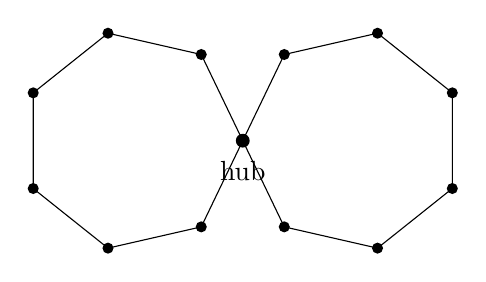
\begin{tikzpicture}[x=0.7cm,y=0.7cm]
\begin{scope}[shift={(-2,0)}]
\coordinate (l0) at (0:2);
\foreach \i in {1,...,6} {\coordinate (l\i) at ({360*\i/7}:2);}
\draw (l0)--(l1)--(l2)--(l3)--(l4)--(l5)--(l6)--cycle;
\foreach \i in {1,...,6} {\fill (l\i) circle (2pt);}
\end{scope}
\begin{scope}[shift={(2,0)}]
\coordinate (r0) at (180:2);
\foreach \i in {1,...,6} {\coordinate (r\i) at ({180+360*\i/7}:2);}
\draw (r0)--(r1)--(r2)--(r3)--(r4)--(r5)--(r6)--cycle;
\foreach \i in {1,...,6} {\fill (r\i) circle (2pt);}
\end{scope}
\fill (0,0) circle (2.5pt) node[below=4pt] {hub};
\end{tikzpicture}
\caption{The support of the order-thirteen seed before the positive completely positive reserve is added. Every proper principal block is completely positive; the full matrix is not.}
\label{fig:bouquet}
\end{figure}

The proof rests on two classical ingredients: a comparison matrix and a bordered Schur complement. We state the exact forms needed, rather than treating the threshold phenomenon as new \cite{Drew,Barioli}.

For a symmetric nonnegative matrix $X$, its \emph{comparison matrix} $M(X)$ keeps the diagonal and negates every off-diagonal entry. Its support graph has an edge $ij$ when $i\ne j$ and $X_{ij}>0$. A graph is triangle-free when no three vertices are pairwise adjacent.

\begin{lemma}[Comparison criterion]\label{lem:comparison}
If $X\ge0$ is symmetric and $M(X)\succeq0$, then $X$ is completely positive. Conversely, if the support graph is triangle-free and $X$ is completely positive, then $M(X)\succeq0$.
\end{lemma}
\begin{proof}
First suppose $M(X)\succ0$. Write $M(X)=tI-K$ with $K\ge0$ and $t>\rho(K)$, taking $t$ sufficiently large. Its inverse is nonnegative by the Neumann series. Thus $d=M(X)^{-1}\mathbf1>0$. The nonnegative matrix $\diag(d)X\diag(d)$ has diagonal excess
\[
 d_i^2X_{ii}-\sum_{j\ne i}X_{ij}d_id_j
 =d_i(M(X)d)_i=d_i>0.
\]
It is therefore the sum of singleton squares with these coefficients and the squares $(e_i+e_j)(e_i+e_j)\T$ with coefficients $X_{ij}d_id_j$. Undoing positive diagonal congruence gives a completely positive factorization of $X$. If $M(X)$ is only semidefinite, apply the result to $X+\eta I$ and let $\eta\downarrow0$, using closedness of $\CP$.

Conversely, in a nonnegative rank-one factorization, a zero entry $X_{ij}=0$ forces every factor to vanish at $i$ or $j$. Each factor is supported on a clique. In a triangle-free graph this support has at most two vertices. Negating the off-diagonal entry of such a rank-one matrix produces another positive semidefinite rank-one matrix. Summing proves $M(X)\succeq0$.
\end{proof}

Let $A_0\in\mathbb S^r(\Q)$ be positive definite and nonnegative, with support a disjoint union of paths and positive edge weights. Singletons are allowed, and components are labeled consecutively. Let $c\in\Q_+^r$ have no two adjacent positive entries. Attaching a hub at these coordinates gives a triangle-free graph $G$. Define
\begin{equation}\label{eq:thresholds}
\begin{gathered}
 M_0=M(A_0),\qquad v=M_0^{-1}c,\qquad
 \alpha=c\T A_0^{-1}c,\qquad \beta=c\T M_0^{-1}c,\\
 F(a)=\begin{pmatrix}A_0&c\\c\T&a\end{pmatrix}.
\end{gathered}
\end{equation}
Changing only the hub diagonal now gives an exact interval. The interval is the constructive route to seeds; its comparison and bordered-matrix antecedents are discussed in \cite{Drew,Barioli}.

\begin{theorem}[Graphical seed interval]\label{thm:seedinterval}
For $a\ge0$,
\[
 F(a)\succ0\quad\Longleftrightarrow\quad a>\alpha,
 \qquad
 F(a)\in\CP_{r+1}\quad\Longleftrightarrow\quad a\ge\beta.
\]
The interval $(\alpha,\beta)$ is nonempty exactly when, in some path component, the hub attaches to both bipartition classes. Under the no-adjacent-attachment assumption, this is equivalent to $G$ containing an odd cycle of length at least five.

For every rational $a$ in this interval, an explicit positive diagonal congruence and completely positive reserve turn $F(a)$ into a certified seed for $T_r$. Hence Theorem~\ref{thm:amplification} applies from $T_{r+1}$ and every bounded region of the same face.
\end{theorem}
\begin{proof}
Give the two classes of each path opposite signs and let $J$ be the resulting diagonal sign matrix. Then $M_0=JA_0J\succ0$. Its inverse is nonnegative, and strictly positive within each connected component: the Neumann series contains a positive walk term between any two connected vertices. The Schur complement of $A_0$ gives the first equivalence. The Schur complement of $M_0$, together with Lemma~\ref{lem:comparison}, gives the second.

If the bipartition is $U\cup V$, sign switching also gives
\begin{equation}\label{eq:thresholdgap}
 \beta-\alpha
 =4\sum_{\substack{i\in U\\j\in V}}c_ic_j(M_0^{-1})_{ij}.
\end{equation}
Terms between different components vanish. The sum is positive precisely when two opposite-colored coordinates are attached in one component. Their path distance is odd; excluding adjacent attachments makes it at least three. Adding the hub produces an odd cycle of length at least five. Conversely, deleting the hub from any cycle leaves the path between its two attachments.

We construct both the separator and the normal reserve. For a triangle-free graph,
\[
 Q_G=\mathbf1\mathbf1\T-2\operatorname{Adj}(G)
\]
is copositive by the Motzkin--Straus bound \cite{MS}. Here is the short argument needed. On the nonnegative simplex, maximize the sum of edge products and choose a maximizer with smallest support. If two positive coordinates are nonadjacent, moving their total mass to the one with larger neighbor sum does not decrease the objective and reduces the support. Thus the support is a clique, of size at most two; its edge product is at most $1/4$. Homogeneity proves copositivity.

Let $W_F=\diag(v,1)Q_G\diag(v,1)$. Using $M_0v=c$ gives the decisive pairing
\begin{equation}\label{eq:graphwitness}
 \ip{W_F}{F(a)}=v\T M_0v-2c\T v+a=a-\beta<0.
\end{equation}
Zero coordinates of $v$ are allowed.

Next set $d=M_0^{-1}\mathbf1>0$ and $D=\diag(d,1)$. The leading block has the exact decomposition
\begin{equation}\label{eq:normalrealization}
 \diag(d)A_0\diag(d)=
 \sum_i d_i e_ie_i\T+
 \sum_{ij\in E(A_0)}(A_0)_{ij}d_id_j(e_i+e_j)(e_i+e_j)\T.
\end{equation}
All displayed vectors minimize $T_r$, since each support edge joins consecutive coordinates. To obtain a spanning positive reserve, let $C_n$ be the sum of all interval squares in order $n=r+1$, as in \eqref{eq:canonicalseed}, and put
\begin{equation}\label{eq:seedassembly}
\begin{gathered}
 W'=D^{-1}W_FD^{-1},\quad \gamma_0=\beta-a,\quad
 w'=1+\sum_{ij}|W'_{ij}|,\quad
 \varepsilon=\frac{\gamma_0}{4w'\tr C_n},\\
 B=DF(a)D+\varepsilon C_n.
\end{gathered}
\end{equation}
This $B$ is rational, positive definite, and strictly positive. Restricting the intervals to the first $r$ coordinates supplies every top interval with positive coefficient.

For completeness,
\begin{equation}\label{eq:Tidentity}
 T_j[x]=\frac12\left(x_1^2+x_j^2+
                 \sum_{i=1}^{j-1}(x_i-x_{i+1})^2\right).
\end{equation}
This is positive for every nonzero real $x$ and is an integer for integer $x$. Its minimum on nonzero nonnegative integer vectors is one, attained at interval indicators. Their squares span: singleton values determine the diagonal, and the four-term difference obtained by deleting either endpoint or both from an interval recovers $2X_{ij}$. Thus $T_r$ is perfect and the reserve meets Definition~\ref{def:seed}. Finally,
$|\ip{W'}{\varepsilon C_n}|\le\varepsilon w'\tr C_n=\gamma_0/4$,
so $\ip{W'}B\le-3\gamma_0/4<0$. The face contains $T_n$ by \eqref{eq:Tidentity}.
\end{proof}

This characterizes the stated graphical class, not arbitrary support graphs. If all attachments lie in one color class per component, \eqref{eq:thresholdgap} vanishes and no hub diagonal gives a positive definite nonmember. Triangle-freeness is also substantive: $J_3$ is completely positive but its comparison matrix $2I-J_3$ is indefinite.

\subsection{All proper principal blocks and a perturbation ball}
To make every proper block pass, choose the hub diagonal just below its full comparison threshold but above every deletion threshold. Let every path component be attached at both endpoints, with any singleton component attached positively. Exclude two-vertex components, which would create triangles, and require at least one component with an even number of vertices $s\ge4$. Then $v=M_0^{-1}c$ is strictly positive and $\beta>\alpha$. Put
\begin{equation}\label{eq:deletionmargins}
 \Delta_i=\frac{v_i^2}{(M_0^{-1})_{ii}}>0,\qquad
 0<\delta<\min\{\beta-\alpha,\min_i\Delta_i\},\qquad
 a=\beta-\delta,
\end{equation}
with all data rational. Half the displayed minimum is one exact choice.

\begin{theorem}[Principal-minimal seeds]\label{thm:minimal}
The matrix $F(a)$ defined above is positive definite, nonnegative, and not completely positive, while every proper principal submatrix is completely positive. The seed $B$ in \eqref{eq:seedassembly} has the same properties and strictly positive entries.

For the interval reserve, choosing $\zeta\le\varepsilon/8$ in \eqref{eq:robustconstants} ensures that every proper principal submatrix of every amplified input in \eqref{eq:ball} is completely positive. Thus no copositive matrix supported on a proper principal index set, nor any nonnegative combination of such matrices, separates these inputs.
\end{theorem}
\begin{proof}
The full Schur complement is $a-\alpha=\beta-\alpha-\delta>0$, but its comparison Schur complement is $a-\beta=-\delta<0$. For deletion of top coordinate $i$, block inversion gives
\begin{equation}\label{eq:deletionidentity}
 \beta-c_{-i}\T(M_0[-i])^{-1}c_{-i}
 =\frac{v_i^2}{(M_0^{-1})_{ii}}=\Delta_i.
\end{equation}
Here $M_0[-i]$ means deletion of row and column $i$. To see the identity directly, partition $M_0$ at $i$; the inverse Schur formula makes the difference the square of the residual component of $c$, divided by the positive scalar Schur complement. Its inverse is $(M_0^{-1})_{ii}$ and its residual divided by that complement is $v_i$, giving the displayed expression.

The comparison matrix of $F(a)[-i]$ has positive Schur complement $\Delta_i-\delta$. It is positive definite and hence $F(a)[-i]$ is completely positive by Lemma~\ref{lem:comparison}. Deleting the hub leaves $A_0$, with positive definite comparison matrix, so that block is also completely positive. Every smaller principal submatrix is contained in a one-coordinate deletion. Positive diagonal congruence and addition of a completely positive matrix preserve all these conclusions. The separator estimate in \eqref{eq:seedassembly} preserves full nonmembership.

We give a uniform radius, including all proper index sets. Regard the interval squares as a basis of $\mathbb S^n$ in upper-triangular coordinates. The inverse coefficient map consists of four-term differences and has maximum absolute row sum at most four. A perturbation $Z$ with $\norm Z_F\le\varepsilon/8$ therefore changes each coefficient of $\varepsilon C_n$ by at most $\varepsilon/2$. All coefficients remain positive, so $\varepsilon C_n+Z$ is completely positive.

For any proper principal set $I$, embed a perturbation of its block by zeros outside $I$, apply the preceding fact, and restrict back to $I$. Adding the already completely positive unreserved principal block proves stability for every $I$ at once. For an amplified perturbation, undo the normalization and the diagonal scaling. Since every diagonal entry of $D_N$ is at least one, its inverse does not increase the Frobenius norm. Thus $\zeta\le\varepsilon/8$ suffices throughout \eqref{eq:ball}.

Finally, complete positivity of $A[I]$ gives $\ip{A[I]}{Q[I]}\ge0$ for every copositive candidate supported on $I$. Summing proves the assertion for nonnegative combinations.
\end{proof}

The order-thirteen numbers can be recovered by a short determinant recurrence. Write $d_k=\det(I_k-\operatorname{Adj}(P_k)/4)$. Then $d_0=d_1=1$ and $d_k=d_{k-1}-d_{k-2}/16$. For $i\le j$, its inverse has entry
\[
 (M_0^{-1})_{ij}=4^{i-j}\frac{d_{i-1}d_{6-j}}{d_6}
\]
on each six-vertex block, with $d_5=195/256$ and $d_6=2911/4096$. Sign switching gives the inverse of $K_6$. Hence one path contributes
\[
 \alpha_0=\frac{152}{71},\qquad \beta_0=\frac{88}{41},\qquad
 \beta_0-\alpha_0=\frac{16}{2911}.
\]
In the two-component matrix, $\min_i\Delta_i=71/8610$. Taking
$\delta=71/17220$ gives exactly $a=73849/17220$ and satisfies \eqref{eq:deletionmargins}. This proves all the claims made above for that example. In particular each seven-cycle principal block passes the completely positive test, while the full matrix fails. Repeating six-vertex components gives examples of unbounded order.

Single even-order paths give another family. With $s\in2\Z$, $s\ge4$, take $A_0=I_s+\operatorname{Adj}(P_s)/4$ and $c=e_1+e_s$. The support is a chordless odd cycle of length $s+1$. Such support obstructions are classical \cite{Kogan}; here they provide qualifying seeds for amplification. Lengths seven and nine have no five-cycle principal support. Weighted nonadjacent attachments and several path components are also covered by Theorem~\ref{thm:seedinterval}; changing the seed's graphical support is separate from the later diagonal amplification.

\subsection{Branched perfect blocks and bounded starting regions}
The leading normal geometry need not be tridiagonal. Let $T$ be a tree with
$H_T=I_r-\operatorname{Adj}(T)/2\succ0$. For every unordered pair, including a repeated pair, let $p_{ij}$ be the indicator of the unique tree path. Then $H_T[p_{ij}]=1$. These are a spanning collection of minimal vectors, not necessarily the complete list. Their squares span $\mathbb S^r$: deleting either endpoint or both from a path gives a four-term difference equal to $2X_{ij}$, and repeated pairs give the diagonal. Since $H_T[x]$ is positive and integral on nonzero integer vectors, $H_T$ is a positive definite perfect vertex.

The same construction works whenever the leading support is a forest contained in $T$. The hypotheses that the hub attachments are nonadjacent and the resulting graph is triangle-free remain in force. The comparison and Schur arguments are unchanged, and the singleton and support-edge vectors in \eqref{eq:normalrealization} are minimal for $H_T$. Use the reserve
\begin{equation}\label{eq:treereserve}
 \mathcal B_T=\sum_{i\le j}\left[
 (p_{ij},0)(p_{ij},0)\T+(p_{ij},1)(p_{ij},1)\T\right]+e_ne_n\T.
\end{equation}
Its leading block is twice the sum of the path squares and all its entries are positive. Its atoms span $\mathbb S^n$: the unlifted paths span the leading block, the final singleton gives the last entry, and lifted singleton paths give the cross entries. Adding $\varepsilon\mathcal B_T$ with $\varepsilon=(\beta-a)/(4w'\tr\mathcal B_T)$ proves the seed conditions exactly as before.

If all proper principal blocks passed before this addition, they still pass and become interior completely positive points. A finite radius is obtained by selecting an atom basis with coefficients at least one in \eqref{eq:treereserve}. If $U$ is its coordinate matrix and $L_U=\norm{U^{-1}}_\infty$, then
$\norm Z_F\le\varepsilon/(2\max(1,L_U))$ preserves positivity of the basis coefficients. The proof of Theorem~\ref{thm:minimal} then gives the principal-block barrier throughout the corresponding amplified ball.

For the branched $D_r$ tree, $r\ge4$, use edges $i(i+1)$ for $1\le i\le r-2$ and $(r-2)r$. The matrix $H_T$ is half the Gram matrix of
$e_1-e_2,\ldots,e_{r-1}-e_r,e_{r-1}+e_r$, so it is positive definite. Adding the new vertex at old vertex $1$ gives a $D_{r+1}$ perfect form with leading block $H_T$, hence an explicit start. On $D_7$, the seed $A_0=I+\operatorname{Adj}(D_7)/4$ with hub attachments at $1$ and $6$ has a seven-cycle and a pendant branch. Choosing its diagonal by \eqref{eq:deletionmargins} gives an order-eight principal-minimal seed. This changes both the seed support and the leading perfect block.

In the canonical face, additional explicit starts are
$P_a=S_a^{-\mathsf T}T_nS_a^{-1}$ for fixed $a\in\Z_+^r$. Indeed $S_a^{-1}(u,y)=(u-ay,y)$ is a nonzero integer vector, and $T_n$ has minimum one on the full integer lattice by \eqref{eq:Tidentity}. Thus $P_a$ is feasible. The forward images $S_a(v,y)=(v+ay,y)$ of the interval minimizers are nonnegative and their squares still span, proving perfectness. Every fixed bounded collection of these starts, and all vertices in any fixed bounded cross-column region of the same face, is covered simultaneously.

\subsection{Further sparsity-limited tests}
A symmetric matrix is called \emph{SPN} if it is a sum of a positive semidefinite matrix and an entrywise nonnegative matrix. A graph is SPN if every copositive matrix with off-diagonal support contained in that graph is SPN. Any copositive candidate confined to such a support has nonnegative pairing with a doubly nonnegative input, regardless of how the candidate is found.

For example, partition the leaf coordinates into groups of at most three. Allow every entry within each group, all hub spokes, and all diagonals. This support is a union of cliques of order at most four meeting only at the hub, and is SPN \cite[Corollaries~4.4 and~5.3]{SPN}. It permits small full-block corrections beyond the diagonal correction in Corollary~\ref{cor:stored}. The forest and small-block results used here are classical and unaffected by the corrigendum \cite{SPNcorr}; no general triangular-book assertion is used.

The new algorithmic consequence of Lemma~\ref{lem:arrow} is simultaneous failure for every stored direction, because confinement puts them all in the arrow space. The principal-minimal seeds supply a different barrier: all proper principal tests fail on the whole certified ball. Neither assertion covers arbitrary off-diagonal corrections or combinations with unrelated non-arrow matrices.
